% ============================================================
% Chapter 8 --- Connectedness
% Originally: content/week-03.tex, \section{Connectedness} (Corsin Week 3, Monday) and
%             \section{Path connectedness} (Corsin Week 3, Friday)
% ============================================================
\chapter{Connectedness}
\label{ch:connectedness}

% Transition: Claude Opus 5 (Medium)
Compactness told us when a space has \qt{enough finiteness} to guarantee extrema and uniform
behaviour. This chapter turns to a completely different, qualitative kind of structure: whether a
space can be split into separate pieces at all. Connectedness and path connectedness are the two
answers, they are not equivalent, and the topologist's sine curve is the standard witness. The
chapter closes with a finer question about paths: whether any two with the same endpoints can be
deformed into each other. That is simple connectedness. Nothing needs it for a long time, but it
returns in the last chapter as the hypothesis that guarantees a curl-free field a potential.
% Transition: Claude Opus 5.5 (Extra) --- the last two sentences; sec:simply_connected is part of
% this chapter and the introduction did not mention it.

% Originally: content/week-03.tex, \section{Connectedness} (Corsin Week 3, Monday)

\section{Connectedness}
\label{sec:connectedness}

\begin{definition}[Connected and disconnected metric spaces]
\label{def:connectedness}
A metric space $(X,d)$ is \newterm{disconnected} \germanfor{unzusammenh\"angend} if there
exist subsets $U_1, U_2 \subseteq X$ which are
\begin{enumerate}[label=\textbf{(\alph*)}]
  \item \textbf{open},
  \item \textbf{non-empty}, $U_1 \neq \emptyset$ and $U_2 \neq \emptyset$,
  \item \textbf{disjoint}, $U_1 \cap U_2 = \emptyset$,
\end{enumerate}
such that $X = U_1 \cup U_2$. Similarly, for a subset $A \subseteq X$, it is disconnected if it is
disconnected as a metric space with the induced metric $d|_{A \times A}$.

If no such pair $U_1, U_2$ exists, $X$ is \newterm{connected}
\germanfor{zusammenh\"angend}. Connected is thus defined as the negation of disconnected.
\end{definition}

Typically, proving that a set or metric space is connected is done \textbf{by contradiction},
which is why one should remember the definition of \textit{disconnected}. Intuitively, connected
means: \qt{the space cannot be separated by open sets.}

\begin{center}
% Generator: Claude Opus 5 (High) --- redrawn. Two things were wrong with the previous
% version. (1) Every $U_i$ label sat directly on a curve --- on the dashed boundary in the
% left panel, on the blob outline in the right --- so all four were unreadable. They are now
% outside their region with a thin leader. (2) The right panel's whole point is that the two
% open sets fail to cover $X$, and it made that point with a 0.14-unit double arrow carrying
% a \tiny "gap" label: at print size an orange smudge, and the gap itself invisible. The gap
% is now a visible strip, with a marked point $p$ of $X$ lying in neither $U_1$ nor $U_2$.
% Feedback: Gemini 3.1 Pro (2026-08-11) --- the redraw was singled out as illustrating the formal
% definition precisely, and the marked point $p$ in the gap by name. Do not shrink the gap back.
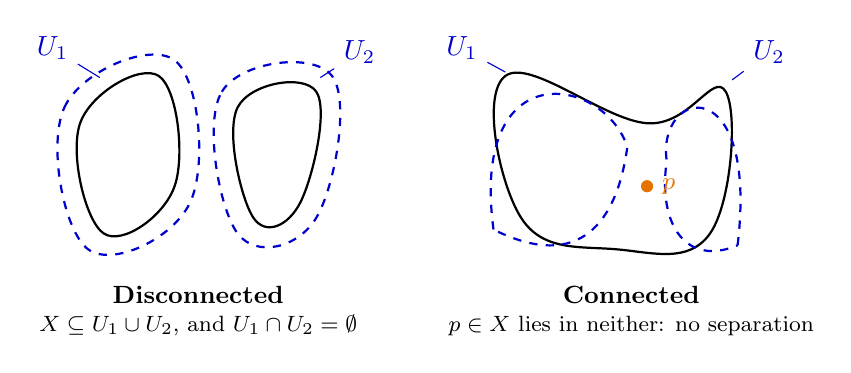
\begin{tikzpicture}[scale=1.0]
  % ---------------- Left panel: Disconnected ----------------
  \begin{scope}[shift={(0,0)}]
    \draw[thick] plot[smooth cycle, tension=0.7] coordinates {(-1.5,-0.8) (-1.8,0.6) (-0.8,1.2) (-0.6,-0.2)};
    \draw[thick] plot[smooth cycle, tension=0.7] coordinates {(0.4,-0.6) (0.2,0.8) (1.2,1.0) (1.0,-0.4)};

    \draw[blue!80!black, thick, dashed] plot[smooth cycle, tension=0.7] coordinates {(-1.7,-1.0) (-2.0,0.8) (-0.6,1.4) (-0.4,-0.4)};
    \node[blue!80!black] (dL) at (-2.15,1.55) {$U_1$};
    \draw[blue!80!black, thin] (dL) -- (-1.55,1.18);

    \draw[blue!80!black, thick, dashed] plot[smooth cycle, tension=0.7] coordinates {(0.2,-0.8) (0.0,1.0) (1.4,1.2) (1.2,-0.6)};
    \node[blue!80!black] (dR) at (1.75,1.5) {$U_2$};
    \draw[blue!80!black, thin] (dR) -- (1.25,1.18);

    \node[below, font=\small, align=center] at (-0.3,-1.35)
      {\textbf{Disconnected}\\[-1pt]{\footnotesize $X \subseteq U_1 \cup U_2$, and $U_1 \cap U_2 = \emptyset$}};
  \end{scope}

  % ---------------- Right panel: Connected ----------------
  % The two dashed regions stop short of one another --- U_1 at x = -0.05, U_2 at x = 0.45 ---
  % leaving a visible vertical strip of X covered by neither. The point p sits in that strip,
  % inside the blob (at x = 0.2 the blob runs from y = -0.95 up to the notch at y = 0.6).
  \begin{scope}[shift={(5.2,0)}]
    \draw[thick] plot[smooth cycle, tension=0.7] coordinates {(-1.4,-0.6) (-1.6,1.2) (0.2,0.6) (1.2,1.0) (1.0,-0.8) (-0.2,-1.0)};

    \draw[blue!80!black, thick, dashed]
      (-1.75,-0.75).. controls (-2.05,1.5) and (-0.35,1.2).. (-0.05,0.30)
      .. controls (-0.18,-0.65) and (-0.65,-1.30).. (-1.75,-0.75);
    \node[blue!80!black] (cL) at (-2.15,1.55) {$U_1$};
    \draw[blue!80!black, thin] (cL) -- (-1.6,1.25);

    \draw[blue!80!black, thick, dashed]
      (1.35,-0.95).. controls (1.62,1.3) and (0.32,1.05).. (0.45,0.12)
      .. controls (0.33,-0.72) and (0.72,-1.22).. (1.35,-0.95);
    \node[blue!80!black] (cR) at (1.75,1.5) {$U_2$};
    \draw[blue!80!black, thin] (cR) -- (1.28,1.15);

    \fill[orange!90!black] (0.2,-0.2) circle (2.2pt);
    \node[orange!90!black, font=\small, right=2pt] at (0.2,-0.2) {$p$};

    \node[below, font=\small, align=center] at (0,-1.35)
      {\textbf{Connected}\\[-1pt]{\footnotesize $p \in X$ lies in neither: no separation}};
  \end{scope}
\end{tikzpicture}
\end{center}

% Generator: Claude (xhigh) --- added because the figure above, the proofs of
% ex:connectedness_tf (a) and (c) and the proof of cor:union_connected_common_point all test a
% subset against disjoint open sets of the whole space, while def:connectedness asks for sets open
% in the subset. Nothing connected the two until now.
The figure draws $U_1$ and $U_2$ as open sets of the surrounding plane, while
\cref{def:connectedness} asks, for a subset, for sets that are open \emph{in the subset}. The two
pictures agree, and several proofs below use the first one.

\begin{lemma}[Separating a subset by open sets of the whole space]
\label{lem:separation_by_ambient_open_sets}
Let $(X,d)$ be a metric space and $A \subseteq X$. Then $A$ is disconnected if and only if there
are open sets $U_1, U_2 \subseteq X$ with
\[A \subseteq U_1 \cup U_2, \qquad U_1 \cap U_2 = \emptyset, \qquad A \cap U_1 \neq \emptyset,
  \qquad A \cap U_2 \neq \emptyset.\]
\end{lemma}

\begin{proof}
\textbf{($\Leftarrow$)} Put $W_i := A \cap U_i$. If $a \in W_i$, some ball $B_\varepsilon(a)$
lies in $U_i$, so the ball of radius $\varepsilon$ about $a$ in $A$, which is
$B_\varepsilon(a) \cap A$, lies in $W_i$. So $W_1$ and $W_2$ are open in $A$, and they are
non-empty, disjoint and cover $A$. They disconnect $A$.

\textbf{($\Rightarrow$)} Let $W_1, W_2$ be open in $A$, non-empty and disjoint, with
$A = W_1 \cup W_2$, and set
\[U_1 := \{x \in X : d(x,W_1) < d(x,W_2)\}, \qquad U_2 := \{x \in X : d(x,W_2) < d(x,W_1)\}.\]
Both are open, since $x \mapsto d(x,W_i)$ is continuous by
\cref{cor:closed_iff_zero_of_distance}, and they are disjoint by construction. Let
$a \in W_1$. Then $d(a,W_1) = 0$, and since $W_1$ is open in $A$ there is $\varepsilon>0$ with
$B_\varepsilon(a) \cap A \subseteq W_1$, so no point of $W_2$ lies within $\varepsilon$ of $a$
and $d(a,W_2) \geq \varepsilon > 0$. Hence $W_1 \subseteq U_1$, and likewise
$W_2 \subseteq U_2$. This gives $A \subseteq U_1 \cup U_2$, with both $U_i$ meeting $A$.
\end{proof}

The work is all in the forward direction. Open sets of $X$ that merely cut $W_1$ and $W_2$ out of
$A$ always exist, but they may overlap away from $A$, and the distance functions are what push
them apart.

% Generator: Claude Opus 5 (High) --- the base case of connectedness, used three times in this
% chapter (path-connectedness, the topologist's sine curve, the intermediate value theorem)
% but stated nowhere in the source notes.
\begin{proposition}[Intervals are connected]
\label{prop:intervals_connected}
Every interval $I \subseteq \mathbb{R}$, whether open, closed, half-open, bounded or unbounded,
is connected (\cref{def:connectedness}). Conversely, a connected subset of $\mathbb{R}$ is an
interval.
\end{proposition}

\begin{proof}
Suppose $I = U_1 \sqcup U_2$ with $U_1, U_2$ open in $I$, disjoint and both non-empty. Pick
$a \in U_1$ and $b \in U_2$; without loss of generality $a<b$, and $[a,b] \subseteq I$ because
$I$ is an interval. Set
\[c := \sup\{\,t \in [a,b] \ :\ [a,t] \subseteq U_1\,\},\]
which is well defined since $a$ belongs to the set. Now $c \in [a,b] \subseteq I$, so $c$ lies
in $U_1$ or in $U_2$, and both lead to a contradiction:
\begin{itemize}
  \item If $c \in U_1$, openness gives $\varepsilon>0$ with $(c-\varepsilon,c+\varepsilon)\cap I
    \subseteq U_1$; together with $[a,c) \subseteq U_1$ this yields $[a,t] \subseteq U_1$ for
    some $t>c$ unless $c=b$, contradicting either the supremum or $b \in U_2$.
  \item If $c \in U_2$, openness gives $\varepsilon>0$ with $(c-\varepsilon,c] \cap I \subseteq
    U_2$. But $c>a$ (as $a \in U_1$ is open in $I$), so by definition of the supremum there is
    $t \in (c-\varepsilon,c]$ with $[a,t] \subseteq U_1$, contradicting disjointness.
\end{itemize}
So no such splitting exists, and $I$ is connected. For the converse, a set $A \subseteq
\mathbb{R}$ that is not an interval admits $a<c<b$ with $a,b \in A$ and $c \notin A$; then
$A \cap (-\infty,c)$ and $A \cap (c,\infty)$ disconnect it.
\end{proof}

\begin{remark}[Why this is the only example one ever needs]
\label{rem:intervals_are_the_base_case}
Every connectedness proof in this chapter reduces to \cref{prop:intervals_connected}: a path is
a continuous image of $[0,1]$ (\cref{def:path}), so path-connected sets are connected
(\cref{lem:path_connected_implies_connected}) purely because the \emph{interval} is; and the
intermediate value theorem, invoked in the topologist's sine curve below, is
\cref{thm:continuity_preserves_connected} applied to an interval, since the connected subsets of
$\mathbb{R}$ are exactly the intervals. In other words, all of it flows from the single fact that
$\mathbb{R}$ has no gaps. That fact is the completeness axiom, and it is what powers the supremum
in the proof above.
\end{remark}

\begin{aiexample}[Disconnectedness of Rational Numbers]
% Generator: Gemini 3.6 Flash (Medium)
The set of rational numbers $\mathbb{Q} \subset \mathbb{R}$ equipped with the subspace topology is disconnected. To see this, define
\[
U := \mathbb{Q} \cap (-\infty, \sqrt{2}) \quad \text{and} \quad V := \mathbb{Q} \cap (\sqrt{2}, \infty).
\]
Since $\sqrt{2} \notin \mathbb{Q}$, we have $U \cup V = \mathbb{Q}$ and $U \cap V = \emptyset$. Both $U$ and $V$ are non-empty and open in the subspace topology of $\mathbb{Q}$ (as intersections of $\mathbb{Q}$ with open intervals in $\mathbb{R}$). Hence $U$ and $V$ form a separation of $\mathbb{Q}$.
\end{aiexample}

% Supplement: Sascha Brack/Class Notes/Week_02_Notes_Friday_Updated.pdf, p. 9
\begin{example}[A disconnected set in $\mathbb{R}^2$]
Let $X := ([0,1] \times [0,1]) \cup ([2,3] \times \{1\}) \subseteq \mathbb{R}^2$. Is $X$ connected?
No. Let $U := \{(x,y) \in X \mid x < 1.5\}$ and $V := \{(x,y) \in X \mid x > 1.5\}$. We can write these as $U = X \cap \{(x,y) \in \mathbb{R}^2 \mid x < 1.5\}$ and $V = X \cap \{(x,y) \in \mathbb{R}^2 \mid x > 1.5\}$. Both $U$ and $V$ are open in the subspace topology of $X$ because they are intersections of $X$ with open half-planes in $\mathbb{R}^2$. Furthermore, $X = U \cup V$, and $U, V$ are disjoint and non-empty. Thus, $X$ is disconnected.
\begin{center}
\begin{tikzpicture}[>=Latex, scale=1.5]
  \draw[->, thick] (-0.2,0) -- (3.5,0);
  \draw[->, thick] (0,-0.2) -- (0,1.5);
  
  \draw[very thick, fill=purple!20, pattern=north east lines, pattern color=purple] (0,0) rectangle (1,1);
  \draw[very thick, purple] (2,1) -- (3,1);
  \node[purple, left] at (-0.1, 0.5) {$X$};
  
  \draw[green!60!black, dashed] (0.5, 0.5) circle (0.8);
  \node[green!60!black] at (1.2, 0.6) {$U$};
  
  \draw[green!60!black, dashed] (2.5, 1) ellipse (0.7 and 0.3);
  \node[green!60!black] at (2.5, 1.4) {$V$};
\end{tikzpicture}
\end{center}
\end{example}

\begin{theorem}[Continuous functions preserve connectedness]
\label{thm:continuity_preserves_connected}
Let $X$, $Y$ be metric spaces, $f : X \to Y$ continuous. If $A \subseteq X$ is connected, then
$f(A)$ is connected.
\end{theorem}

% Generator: Claude Opus 5 (High) --- stated without proof in the source; the argument is three
% lines and is the exact dual of \cref{item:continuity_preserves_compact}.
\begin{proof}
We may assume $A = X$, replacing $X$ by $A$ with the induced metric and $Y$ by $f(A)$. Suppose
$f(X)$ were disconnected, say $f(X) = V_1 \sqcup V_2$ with $V_1,V_2$ open in $f(X)$, disjoint
and non-empty. Then $U_i := f^{-1}(V_i)$ is open by \cref{def:continuous}\textbf{(c)},
non-empty because $V_i$ meets the image, and $U_1 \cap U_2 = \emptyset$ with
$U_1 \cup U_2 = X$ because the $V_i$ partition $f(X)$. So $U_1,U_2$ disconnect $X$, contrary to
hypothesis.
\end{proof}

\begin{corollary}[Intermediate value theorem]
\label{cor:intermediate_value_theorem}
Let $f : [a,b] \to \mathbb{R}$ be continuous. Then $f$ attains every value between $f(a)$ and
$f(b)$.
\end{corollary}

\begin{proof}
By \cref{prop:intervals_connected}, $[a,b]$ is connected, so $f([a,b])$ is connected by
\cref{thm:continuity_preserves_connected}, hence is an interval (\cref{prop:intervals_connected}
again). An interval containing $f(a)$ and $f(b)$ contains everything between them.
\end{proof}

% Reclassified from ainote to plain prose: this says why the corollary is worth stating, which
% is a mathematical judgement, not a note about the transcription.
% Transition: Claude Opus 5 (High)
The intermediate value theorem is a result from \emph{Analysis I}, and re-deriving it here costs
one line. It is worth the line twice over. This is the first place where connectedness earns its
keep, and the derivation makes visible that the theorem is really a statement about $\mathbb{R}$
having no gaps rather than a statement about $f$. It is used again in the topologist's sine curve
(\cpageref{ex:topologists_sine_curve}) below.

% Supplement: Analysis_II_Script_v1.pdf, p. 29
\begin{corollary}[Intermediate value theorem on a connected space]
\label{cor:ivt_general_connected}
Let $X$ be a connected metric space and $f : X \to \mathbb{R}$ continuous. For any $a,b \in X$
and any $y \in \mathbb{R}$ between $f(a)$ and $f(b)$, there exists $x \in X$ with $f(x) = y$.
\end{corollary}

\begin{proof}
Word for word \cref{cor:intermediate_value_theorem}'s proof, with $X$ in place of $[a,b]$: $X$
is connected by hypothesis (rather than by \cref{prop:intervals_connected}), so $f(X)$ is
connected by \cref{thm:continuity_preserves_connected}, hence an interval by
\cref{prop:intervals_connected}; an interval containing $f(a)$ and $f(b)$ contains everything
between them.
\end{proof}

\begin{remark}
\Cref{cor:intermediate_value_theorem} is the special case $X = [a,b]$. Stating the general
version separately is worth doing once: it makes clear that connectedness, not any special
property of an interval, is what the intermediate value theorem actually needs. That is exactly
the moral of \cref{rem:intervals_are_the_base_case}.
\end{remark}

% Supplement: Sascha Brack/Class Notes/Week_03_Notes_Monday.pdf, p. 4
% Retitled by Claude Opus 5.5 (Extra): "Linear maps preserve the unit cube" claimed more than the
% statement, which says the image is a (possibly degenerate) parallelepiped, connected and compact.
\begin{corollary}[Linear images of the unit cube are connected and compact]
\label{cor:linear_maps_unit_cube}
% Correction: Claude Opus 5 (Ultracode) --- read "maps $[0,1]^n$ to an $n$-dimensional
% parallelepiped", which fails for every singular $L$: at $L = 0$ the image is a single point.
% Qualified as possibly degenerate, the way ex:equations_to_drawings part (e) already handles the
% same collapse in the plane. The two claims the corollary is actually for, connected and
% compact, hold for every $L$ and are untouched.
Given the $n$-dimensional unit cube $[0,1]^n \subset \mathbb{R}^n$, any linear map $L : \mathbb{R}^n \to \mathbb{R}^n$ maps $[0,1]^n$ to a parallelepiped, possibly degenerate: if $L$ is singular the image collapses to a parallelepiped of lower dimension, and to the single point $\{0\}$ when $L = 0$. Since linear maps in Euclidean space are continuous, the image $L([0,1]^n)$ is connected. Furthermore, since $[0,1]^n$ is compact, $L([0,1]^n)$ is also compact.
\end{corollary}

\begin{exercise}[Properties of connectedness]
\label{ex:connectedness_tf}
Are the following true or false?
\begin{enumerate}[label=\textbf{(\alph*)}]
  \item The union of connected subsets with a common point is connected.
  \item The intersection of connected subsets is connected.
  % Not a first introduction -- \newterm/\germanterm for "closure" belong to
  % \cref{def:interior_closure_boundary}, so this is a plain back-reference.
  \item The closure (\cref{def:interior_closure_boundary}) of a connected subset is connected.
\end{enumerate}
\end{exercise}

% Kept inline: solved directly in Corsin Nick/Class Notes/Week 3.pdf, pp. 5--6.
\begin{exercisesolution}[Proof of \cref{ex:connectedness_tf}]
\textbf{(a) True.} \textit{Proof.} Let $X$ be a metric space, $V_1, V_2 \subseteq X$ connected,
and $x_0 \in V_1 \cap V_2$. Suppose $V_1 \cup V_2 \subseteq U_1 \cup U_2$ with
$U_1, U_2 \subseteq X$ open and disjoint. By \cref{lem:separation_by_ambient_open_sets} it is
enough to show that one of them misses $V_1 \cup V_2$. Assume without loss of generality
$x_0 \in U_1$. Then $U_1 \cap V_1 \neq \emptyset$ and $U_1 \cap V_2 \neq \emptyset$. So, since
$V_1, V_2$ are connected, \cref{lem:separation_by_ambient_open_sets} gives
$V_1 \cap U_2 = V_2 \cap U_2 = \emptyset$. Therefore $(V_1 \cup V_2) \cap U_2 = \emptyset$ and
$V_1 \cup V_2$ is connected.

\textbf{(b) False.} \textit{Counterexample:}
\[
X = \mathbb{R}^2, \quad U = [-1,1] \times \{0\}, \quad V = S^1 = \{x \in \mathbb{R}^2 : |x| = 1\},
\]
\[
U \cap V = \{(-1,0), (1,0)\}.
\]

\textbf{(c) True.} Suppose $X$ is a metric space, $A \subseteq X$ a subset with closure
$\overline{A}$. Suppose $U_1, U_2 \subseteq X$ are disjoint open sets covering $\overline{A}$, and
assume without loss of generality $\overline{A} \cap U_1 \neq \emptyset$. Then, since $U_1$ is
open, $A \cap U_1 \neq \emptyset$. By connectedness of $A$ and
\cref{lem:separation_by_ambient_open_sets}, $U_2 \cap A = \emptyset$, and since $U_2$ is open,
also $U_2 \cap \overline{A} = \emptyset$. So no such pair separates $\overline{A}$, which is
therefore connected by \cref{lem:separation_by_ambient_open_sets} once more.
\end{exercisesolution}

\begin{ainote}
Corsin writes $|x| = R^2$ in the definition of $S^1$ above; it must be $|x| = 1$, as the
stated intersection $\{(\pm 1, 0)\}$ confirms. Corrected here.
\end{ainote}

% Correction: Claude (xhigh) --- the proofs of (a) and (c) tested connectedness against disjoint
% open sets of X without saying why that is the same as def:connectedness; they now cite
% lem:separation_by_ambient_open_sets at each step that needs it.
\begin{ainote}
Corsin's proofs of \textbf{(a)} and \textbf{(c)} test connectedness against disjoint open sets of
the whole space $X$, whereas \cref{def:connectedness} asks for sets open in the subset. The two
tests agree, but only by \cref{lem:separation_by_ambient_open_sets}, which his notes do not
state. His arguments are unchanged above, and the references to the lemma are added.
\end{ainote}

\begin{center}
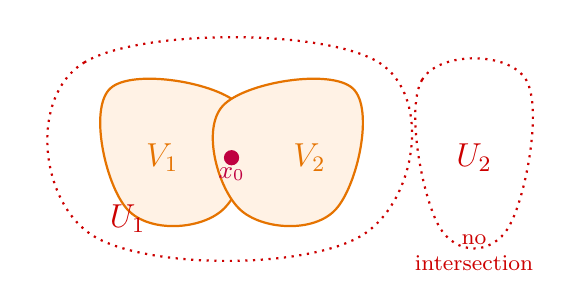
\begin{tikzpicture}[scale=1.1]
  \draw[orange!90!black, thick, fill=orange!10] plot[smooth cycle, tension=0.7] coordinates {(-1.6,-0.6) (-1.8,0.8) (-0.3,0.6) (-0.5,-0.6)};
  \node[orange!90!black, font=\large] at (-1.2,0) {$V_1$};

  \draw[orange!90!black, thick, fill=orange!10] plot[smooth cycle, tension=0.7] coordinates {(-0.3,-0.6) (-0.5,0.6) (1.0,0.8) (0.8,-0.6)};
  \node[orange!90!black, font=\large] at (0.5,0) {$V_2$};

  \fill[purple] (-0.4,0) circle (2.5pt) node[below, font=\small] {$x_0$};

  \draw[red!80!black, thick, dotted] plot[smooth cycle, tension=0.7] coordinates {(-2.0,-0.9) (-2.1,1.1) (1.3,1.1) (1.1,-0.9)};
  \node[red!80!black, font=\large] at (-1.6,-0.7) {$U_1$};

  \draw[red!80!black, thick, dotted] plot[smooth cycle, tension=0.7] coordinates {(2.0,-0.8) (1.8,0.9) (3.0,0.9) (2.8,-0.8)};
  \node[red!80!black, font=\large] at (2.4,0) {$U_2$};
  \node[red!80!black, font=\footnotesize, align=center] at (2.4,-1.1) {no\\intersection};
\end{tikzpicture}
\end{center}

\begin{center}
\begin{tikzpicture}[>=Latex, scale=1.3]
  \draw[->] (-1.6,0) -- (1.6,0) node[right] {$x$};
  \draw[->] (0,-1.6) -- (0,1.6) node[above] {$y$};

  \draw[red!80!black, thick] (0,0) circle (1.0);
  \node[red!80!black, above right] at (0.7,0.7) {$S^1$};

  \draw[orange!90!black, ultra thick] (-1,0) -- (1,0);
  \node[orange!90!black, below] at (0,-0.1) {$U = [-1,1]\times\{0\}$};

  \fill[purple] (-1,0) circle (2pt) node[above left, font=\footnotesize] {$(-1,0)$};
  \fill[purple] (1,0) circle (2pt) node[above right, font=\footnotesize] {$(1,0)$};
\end{tikzpicture}
\end{center}

% Supplement: Analysis_II_Script_v1.pdf, p. 28
\begin{corollary}[Arbitrary unions of connected sets through a common point]
\label{cor:union_connected_common_point}
Let $(X,d)$ be a metric space, $p \in X$, and $\{V_i\}_{i\in I}$ a family of connected subsets of
$X$ with $p \in V_i$ for every $i \in I$. Then $\bigcup_{i\in I}V_i$ is connected.
\end{corollary}

% Correction: Claude (xhigh) --- now says that separations by disjoint open sets of X are enough,
% which is lem:separation_by_ambient_open_sets.
\begin{proof}
By \cref{lem:separation_by_ambient_open_sets} it suffices to rule out disjoint open sets
$U_1, U_2 \subseteq X$ that cover the union and both meet it. So suppose
$\bigcup_i V_i \subseteq U_1 \cup U_2$ with $U_1,U_2$ open and disjoint, and say
$p \in U_1$. For each $i$, the argument of \cref{ex:connectedness_tf}\textbf{(a)} applies to
$V_i$ alone: it meets $U_1$ (at $p$) and is connected, so it cannot also meet $U_2$, i.e.\
$V_i \subseteq U_1$. This holds for every $i \in I$, so $\bigcup_i V_i \subseteq U_1$, and $U_2$
cannot meet $\bigcup_i V_i$: no separation of the union exists.
\end{proof}

\begin{definition}[Connected component]
\label{def:connected_component}
Let $(X,d)$ be a metric space and $x \in X$. The \newterm{connected component}
\germanfor{Zusammenhangskomponente} of $x$ is
\[C_x := \bigcup\{V \subseteq X : V \text{ connected and } x \in V\},\]
the union of all connected subsets of $X$ containing $x$.
\end{definition}

\begin{remark}
By \cref{cor:union_connected_common_point} (with $I$ indexing \emph{all} connected sets
containing $x$, and common point $p := x$), $C_x$ is itself connected. It is therefore the
\emph{largest} connected subset of $X$ containing $x$, since it contains every connected set
that does. Two connected components are either equal or disjoint: if $C_x \cap C_y \neq
\emptyset$, pick $p$ in the intersection; then $C_x \cup C_y$ is connected
(\cref{cor:union_connected_common_point} again, common point $p$) and contains both $x$ and $y$,
so maximality of $C_x$ and $C_y$ forces $C_x \cup C_y \subseteq C_x$ and
$C_x \cup C_y \subseteq C_y$, that is, $C_x = C_y$. Hence the connected components partition $X$
into disjoint pieces, which is the connectedness analogue of the way an equivalence relation
partitions a set into equivalence classes.
\end{remark}

% Source: Jérôme Paschoud/Notizen/Woche 3.2 Zusammenhängende Mengen.pdf, p. 3
% Generator: Gemini 3.6 Flash (High)
\begin{remark}[Summary of topological properties under continuous maps]
\label{rem:summary_continuous_maps}
Let $X,Y$ be metric spaces and $f: X \to Y$ a continuous function. The following table summarizes which topological properties of a subset $A \subseteq X$ or $B \subseteq Y$ are necessarily preserved under images $f(A)$ and preimages $f^{-1}(B)$.

\begin{center}
\begin{tabular}{@{}l c c@{}}
If $A$ or $B$ is \dots & Then $f^{-1}(B)$ is \dots & Then $f(A)$ is \dots \\
open & \textbf{open} & (not necessarily) \\
closed & \textbf{closed} & (not necessarily) \\
compact & (not necessarily) & \textbf{compact} \\
connected & (not necessarily) & \textbf{connected}
\end{tabular}
\end{center}
\end{remark}

% Source: old_exams/examHS24.pdf (13 February 2025), Kästchenaufgabe 1, p. 7
% Extractor: Claude Opus 5 (High)
\begin{exercise}[Connected but not simply connected]
\label{ex:closed_unbounded_not_simply_connected}
Give an example of a subset $U \subseteq \mathbb{R}^2$, with the Euclidean distance, that is closed
and unbounded, connected, but \emph{not} simply connected. Justify each of the four properties.
\exinfo{This exercise is taken from the exam of 13 February 2025 (Prof.\ Joaquim Serra), Box Problem 1, where only the
final answer was graded.}
\exsol{sol:closed_unbounded_not_simply_connected}
\end{exercise}

% Source: old_exams/examHS24.pdf (13 February 2025), Wahr/Falsch-Fragen, Aufgabe 1, p. 2
% Extractor: Gemini 3.1 Pro (High)
\begin{exercise}[True or False \textnormal{(topology and continuous images)}]
\label{ex:examHS24_TF_topology}
Let $U = \{ (x,y) \in \mathbb{R}^2 : -x^2 \le y \le x^2 \}$ and $f(x,y) = \frac{x^2}{1+y^2}$.
Decide whether each of the following statements is true or false.
\begin{enumerate}[label=\textbf{(\alph*)}]
  \item $U$ is closed.
  \item $U$ is simply connected.
  \item $U$ is compact.
  \item $f(U) \subseteq \mathbb{R}$ is connected.
  \item $f$ is bounded.
  \item There exists a point $p \in U$ such that $f(p) = \inf\{f(q) \mid q \in U\}$.
\end{enumerate}
\exinfo{This exercise is taken from the exam of 13 February 2025 (Prof.\ Joaquim Serra), where it appears as the first
block of true/false questions.}
\exsol{sol:topology_continuous_images_tf}
\end{exercise}

% Source: exercises_2024/mock.pdf (Analysis II mock examination, Spring Semester 2024,
% Prof. Joaquim Serra), Box Problem 19, p. 3
% Extractor: Claude Opus 5 (High)
% The section proves that a union of connected sets with a common point is connected, and says
% nothing about intersections, for the good reason that there is nothing to say. This asks the
% reader to supply the reason in a picture.
\begin{exercise}[Box question: connected union, disconnected intersection]
\label{ex:box_intersection_disconnected_union_connected}
Sketch two open connected sets $U_1, U_2 \subseteq \mathbb{R}^2$ such that $U_1 \cap U_2$ is
\emph{not} connected while $U_1 \cup U_2$ is connected, and justify all four claims.
\exinfo{This exercise is taken from the mock examination for Analysis II, Spring Semester 2024
(Prof.\ Joaquim Serra), Box Problem 19, where only the final answer was graded. The request for
justifications is added here.}
\exsol{sol:box_intersection_disconnected_union_connected}
\end{exercise}

% Originally: content/week-03.tex, \section{Path connectedness} (Corsin Week 3, Friday)

\section{Path connectedness}
\label{sec:path_connectedness}

% Transition: Claude Opus 5 (High)
\Cref{def:connectedness} defines connectedness negatively. A space is connected when it
\emph{cannot} be split, which is why proofs about it run by contradiction. That is mathematically
convenient and intuitively unsatisfying, since it says nothing whatever about what holds a
connected space together.

Path connectedness is the positive version, and it says the obvious thing: any two points can be
joined by a curve running inside the space. It implies connectedness
(\cref{lem:path_connected_implies_connected}), and on open subsets of $\mathbb{R}^n$ the two
notions agree (\cref{prop:open_euclidean_connected_path_connected}). In general they come apart,
and the topologist's sine curve at the end of this section is the standard witness.

% Source: Corsin Nick/Class Notes/Week 3.pdf, pp. 1--14
\begin{definition}[Path]
\label{def:path}
Let $(X,d)$ be a metric space. A continuous function $\gamma : [0,1] \to X$, where $[0,1]$
carries the standard metric, is called a \newterm{path} \germanfor{Weg}. More generally, we
can replace $[0,1]$ by $[a,b]$ for $a < b$.
\end{definition}

\begin{definition}[Path-connected]
\label{def:path_connected}
A metric space $X$ (or subset thereof) is \newterm{path-connected}
\germanfor{wegzusammenh\"angend} if for all $x, y \in X$ there exists a path
(\cref{def:path}) $\gamma : [0,1] \to X$ with $\gamma(0) = x$, $\gamma(1) = y$.
\begin{center}
\begin{tikzpicture}[>=Latex]
  \draw[very thick, fill=gray!10] plot[smooth cycle, tension=0.7] coordinates {(-2, -1) (-2.5, 0.5) (-1, 1.5) (1.5, 1) (2.5, -0.5) (1, -1.5)};
  \node[font=\large] at (2, 0.8) {$X$};
  
  \fill (-1.5, -0.2) circle (1.5pt) node[below] {$x$};
  \fill (1.8, -0.1) circle (1.5pt) node[below] {$y$};
  
  \draw[blue, thick, ->] (-1.5, -0.2) .. controls (-1, 1) and (1, -1) .. (1.8, -0.1);
  
  \node[blue, above] at (-1.5, -0.2) {$\gamma(0)$};
  \node[blue, above] at (1.8, -0.1) {$\gamma(1)$};
  \node[blue, below] at (0, -0.1) {$\gamma([0,1])$};
\end{tikzpicture}
\end{center}
\end{definition}

\begin{lemma}[Path-connected implies connected]
\label{lem:path_connected_implies_connected}
Let $X$ be a metric space. Then $X$ path-connected (\cref{def:path_connected}) implies $X$
connected (\cref{def:connectedness}).
\end{lemma}

% Generator: Claude Opus 5 (High) --- stated without proof in the source.
\begin{proof}
Suppose $X$ were path-connected but disconnected, say $X = U_1 \sqcup U_2$ with $U_1,U_2$ open,
disjoint and non-empty. Pick $x \in U_1$, $y \in U_2$ and a path $\gamma : [0,1] \to X$ with
$\gamma(0)=x$, $\gamma(1)=y$. Then $\gamma^{-1}(U_1)$ and $\gamma^{-1}(U_2)$ are open in $[0,1]$
by \cref{def:continuous}\textbf{(c)}, disjoint, cover $[0,1]$, and are non-empty (they contain
$0$ and $1$ respectively). This disconnects $[0,1]$, contradicting
\cref{prop:intervals_connected}.
\end{proof}

% Source: Jérôme Paschoud/Notizen/Woche 3.1 Banach und Kompaktheit.pdf, p. 6
% Generator: Gemini 3.6 Flash (High)
\begin{exercise}[The unit disk is connected]
\label{ex:disk_connected}
Prove that the set $S^1 := \{ (x,y) \in \mathbb{R}^2 \mid x^2 + y^2 \leq 1 \}$ is connected.
\end{exercise}

\begin{exercisesolution}[Proof of \cref{ex:disk_connected}]
Instead of proving connectedness directly via open sets, we can show that $S^1$ is path-connected, which implies connectedness (\cref{lem:path_connected_implies_connected}). Given any two points $a, b \in S^1$, we can connect them via a straight line segment. The segment can be parameterized as $\gamma(t) := (1-t)a + tb$ for $t \in [0,1]$. Since $S^1$ (the unit disk in $\mathbb{R}^2$) is convex, for any $t \in [0,1]$ we have $|\gamma(t)| \leq (1-t)|a| + t|b| \leq 1-t + t = 1$, so the entire path lies in $S^1$. Because any two points can be connected by a continuous path within $S^1$, the set is path-connected, and therefore connected.

(Note: The standard notation for the unit disk is $D^2$ or $B_1(0)$, whereas $S^1$ usually denotes the boundary circle $\{x^2+y^2=1\}$, but we reproduce the notation $S^1$ here as it appears in the source notes.)
\end{exercisesolution}

\begin{proposition}[Connectedness and path-connectedness in open Euclidean subsets]
\label{prop:open_euclidean_connected_path_connected}
Let $U \subseteq \mathbb{R}^n$ be open (\cref{def:open_closed}). Then
\[
U \text{ path-connected} \iff U \text{ connected}.
\]
\end{proposition}

% Generator: Claude Opus 5 (High) --- stated without proof in the source; the "(<=)" direction
% is the standard "the set of reachable points is clopen" argument and is worth having, since it
% is the only place in this chapter where openness is genuinely used.
\begin{proof}
\textbf{($\Rightarrow$)} is \cref{lem:path_connected_implies_connected}, which needs neither
openness nor $\mathbb{R}^n$.

\textbf{($\Leftarrow$)} Assume $U$ is connected and non-empty (the empty set is vacuously
path-connected), and fix $x_0 \in U$. Let
\[A := \{x \in U \ :\ \text{some path in } U \text{ joins } x_0 \text{ to } x\}.\]
We show $A$ and $U \setminus A$ are both open; since $x_0 \in A$ (take the constant path),
connectedness then forces $U\setminus A = \emptyset$, i.e.\ $A = U$, which is the claim.

Let $x \in U$ and choose $r>0$ with $B_r(x) \subseteq U$, using that $U$ is open. The ball is
convex, so every $y \in B_r(x)$ is joined to $x$ by the straight segment
$t \mapsto (1-t)x+ty$, which stays inside $B_r(x) \subseteq U$. Consequently:
\begin{itemize}
  \item If $x \in A$, concatenating a path from $x_0$ to $x$ with that segment joins $x_0$ to
    any $y \in B_r(x)$, so $B_r(x) \subseteq A$ and $A$ is open.
  \item If $x \notin A$, then no $y \in B_r(x)$ can lie in $A$, since otherwise running the
    segment backwards from $y$ to $x$ would join $x_0$ to $x$. So $B_r(x) \subseteq U\setminus A$ and
    $U\setminus A$ is open.
\end{itemize}
(Concatenation of two paths is again a path: traverse the first on $[0,\tfrac12]$ and the second
on $[\tfrac12,1]$, each at double speed; the result is continuous because the two pieces agree
at $t=\tfrac12$.)
\end{proof}

\begin{importantremark}[Only for open subsets]
\label{rem:path_connected_needs_open}
The implication \qt{connected $\Rightarrow$ path-connected} is \emph{false} without openness,
and the proof shows exactly why: the ball $B_r(x)$ around a point of $U$ was needed to supply
the straight segment. For a set that is not open there may be points with no room around them at
all, and the topologist's sine curve (\cref{ex:topologists_sine_curve}) below is precisely such
a case. There the origin has no neighbourhood in $S$ that is a nice piece of curve.
\end{importantremark}

% Source: Corsin Nick/Class Notes/Week 3.pdf, pp. 1--14
% (Re-cited: the two proofs and the important remark above are additions, not transcription.)
\begin{example}[The topologist's sine curve]
\label{ex:topologists_sine_curve}
\[S := \left\{\left(t, \sin\left(\tfrac{1}{t}\right)\right) : t > 0\right\} \cup \{(0,0)\} \subseteq \mathbb{R}^2\]
$S$ is \textbf{connected} but \textbf{not path-connected}!
\end{example}

\begin{ainote}
Corsin writes the second piece as $\cup\,\{0\}$; since $S \subseteq \mathbb{R}^2$, the point
being adjoined is the origin $(0,0) \in \mathbb{R}^2$, not the number $0$. Written as
$\cup\,\{(0,0)\}$ above, which is also what his own figure and the proof below use.
\end{ainote}

\begin{center}
\begin{tikzpicture}[>=Latex, scale=1.3]
  \draw[->] (-0.2,0) -- (3.2,0) node[right] {$t$};
  \draw[->] (0,-1.4) -- (0,1.4) node[above] {$y$};
  \draw (0,1.0) -- (-0.05,1.0) node[left, font=\footnotesize] {$1$};
  \draw (0,-1.0) -- (-0.05,-1.0) node[left, font=\footnotesize] {$-1$};
  % Horizontal figure-coordinate \x corresponds to t = \x/10, since the plot is sin(10/\x).
  \draw (1.0,0.05) -- (1.0,-0.05) node[below, font=\footnotesize] {$0.1$};
  \draw (2.0,0.05) -- (2.0,-0.05) node[below, font=\footnotesize] {$0.2$};

  \draw[blue!80!black, thick] plot[domain=0.08:2.8, samples=250] (\x, {sin((1.0/(\x*0.1)) r)});
  \fill[blue!80!black] (0,0) circle (1.5pt) node[left, font=\footnotesize] {$(0,0)$};
  \node[above, font=\small] at (1.5,1.3) {$S = \{(t, {\sin(1/t})) : t > 0\} \cup \{(0,0)\}$};
\end{tikzpicture}
\end{center}

\begin{proof}[$S$ is connected]
Write $G := S \setminus \{(0,0)\} = \{(t,\sin(1/t)) : t>0\}$ for the graph part, and suppose for
contradiction that $S$ is disconnected, say $S = V_1 \sqcup V_2$ with $V_1,V_2$ non-empty,
disjoint and open in $S$. Say $(0,0) \in V_1$.

$G$ is the continuous image of the interval $(0,\infty)$ under
$t \mapsto (t,\sin(1/t))$, hence path-connected, hence connected
(\cref{lem:path_connected_implies_connected}). A connected set meeting both parts of a
separation would itself be separated, so $G$ lies entirely in $V_1$ or entirely in $V_2$.

It cannot lie in $V_1$: then $V_2 \subseteq S \setminus (G \cup \{(0,0)\}) = \emptyset$,
contradicting $V_2 \neq \emptyset$. So $G \subseteq V_2$, and therefore
$V_1 = \{(0,0)\}$.

But $V_1$ is open in $S$, so some ball $B_\varepsilon\big((0,0)\big) \cap S$ equals
$\{(0,0)\}$, and that is false. For $t := \tfrac{1}{k\pi}$ with $k$ large, the point
$(t,\sin(1/t)) = (t,0) \in G$ lies within $\varepsilon$ of the origin. This is the required
contradiction, so $S$ is connected.
\end{proof}

\begin{proof}[$S$ is not path-connected]
Assume by contradiction there is a path from $(0,0)$ to $(\tfrac{1}{\pi}, 0)$,
\[
\gamma : [0,1] \to S, \qquad t \mapsto (x(t), y(t)).
\]
Since $\gamma$ is continuous, $x$ and $y$ must also be continuous. By the \newterm{intermediate
value theorem} (\cref{cor:intermediate_value_theorem}), $x : [0,1] \to [0,\infty)$
attains every value in $[0,\tfrac{1}{\pi}]$, since $x(0) = 0$ and $x(1) = \tfrac{1}{\pi}$.
Therefore, we find a sequence $(a_n)_{n=1}^{\infty}$ such that
\[
x(a_n) = \frac{1}{2\pi n + \tfrac{\pi}{2}}.
\]
We may moreover choose the $a_n$ \textbf{decreasing}: having found $a_{n-1}$, apply the
intermediate value theorem on $[0,a_{n-1}]$ rather than on $[0,1]$, which is legitimate because
$x(0) = 0$ and $x(a_{n-1}) = \tfrac{1}{2\pi(n-1)+\pi/2}$ already straddle the next target value.
This yields $a_n \in (0,a_{n-1})$, so $(a_n)$ is decreasing and bounded below, hence convergent,
say $a_n \to \ell \in [0,1]$.

Now evaluate $\gamma$ along this sequence. By construction $x(a_n) \to 0$, so continuity gives
$x(\ell) = 0$; and $y(a_n) = \sin\!\big(2\pi n + \tfrac\pi2\big) = 1$ for every $n$, so
$y(\ell) = 1$. Hence $\gamma(\ell) = (0,1)$. But $(0,1) \notin S$: the only point of $S$ whose
first coordinate vanishes is the origin. This contradicts $\gamma([0,1]) \subseteq S$, so no
such path exists.
\end{proof}

% Feedback: Gemini 3.1 Pro (2026-08-11) --- flagged as a genuine proof gap correctly closed: the
% $a_n$ have to be produced on shrinking intervals $[0,a_{n-1}]$ or they need not tend to $0$.
% Do not quietly drop this note; it is what records the divergence from Corsin's PDF.
\begin{ainote}
Corsin's argument produces the $a_n$ from the intermediate value theorem and then asserts
$a_n \to 0$. That does not follow from the choice as stated. The intermediate value theorem
returns \emph{some} preimage, and nothing so far prevents all of them from sitting near $1$.
The repair is the standard one and costs one sentence: apply the theorem on the shrinking
intervals $[0,a_{n-1}]$ rather than on $[0,1]$ each time, which forces the $a_n$ down. Inserted
above; the rest of his proof is unchanged.
\end{ainote}

\begin{center}
\begin{tikzpicture}[>=Latex, scale=1.3]
  \draw[->] (-0.3,0) -- (3.2,0) node[right] {$t$};
  \draw[->] (0,-1.4) -- (0,1.4) node[above] {$y$};

  \draw[blue!80!black, thick] plot[domain=0.08:2.8, samples=250] (\x, {sin((1.0/(\x*0.1)) r)});

  \fill[red!80!black] (0,0) circle (2pt) node[below left, font=\small] {$\gamma(0)$};

  % The peaks of the plotted sin(10/x) sit at x = 20/(pi(1+4k)), k = 1,2,3,...
  % -- these must land ON the curve, since they are the points gamma(a_n).
  \fill[red!80!black] (1.273,1.0) circle (2pt) node[above right, font=\footnotesize] {$\gamma(a_1)$};
  \fill[red!80!black] (0.707,1.0) circle (1.7pt);
  \fill[red!80!black] (0.490,1.0) circle (1.4pt);
  \fill[red!80!black] (0.374,1.0) circle (1.1pt);
  \fill[red!80!black] (0.303,1.0) circle (0.9pt);

  % The limit (0,1) is NOT a point of S -- hence the hollow circle.
  \draw[red!80!black, thick] (0,1.0) circle (2.5pt);
  \node[red!80!black, font=\footnotesize, left] at (-0.08,1.0) {$(0,1)$};
  \draw[red!80!black, ->, dashed] (1.15,1.19) -- (0.13,1.07);

  \node[red!80!black, font=\small] at (1.75,-1.15) {$\gamma(a_n) \to (0,1) \neq (0,0) = \gamma(0)$};
\end{tikzpicture}
\end{center}

\subsection{Simple connectedness}
\label{sec:simply_connected}

% Supplement: lec_notes.pdf, Definition 14.89, printed p. 200
% Generator: Claude Opus 5 (High)
% Gap closed 2026-08-11. "Simply connected" was used in three exercises of chapters 7 and 8
% (ex:annulus_continuous_image, ex:closed_unbounded_not_simply_connected, ex:examHS24_TF_topology)
% and defined nowhere before chapter 26, where it appeared only informally, inside an ainote
% attached to cor:potentials_simply_connected. The definition below is Definition 14.89, and the
% ainote in 26-stokes/03-poincare-lemma.tex now points here instead of redefining the term.
% NOTE: the lecture notes flag section 14.5.3 and this definition as "[Extra material]". Kept
% anyway, and the scope rule in gemini.md is not being violated: this is not a new section for a
% skipped topic but a definition for a term three of our own exercises already use, and it is
% examined --- 21 August 2024 asks whether an annulus is simply connected (Aufgabe 1.2) and both
% Serra papers close with a true/false block on closed-but-not-exact fields.
Connectedness asks whether a set falls into separate pieces, and path-connectedness asks whether
any two points can be joined. Neither notices a \emph{hole}: an annulus is connected and
path-connected, and yet a loop running around its inner boundary cannot be shrunk to a point
without leaving the set. The third notion in the family is the one that sees this, and it is
needed as early as \cref{ex:annulus_continuous_image}, well before the chapter on the Poincaré
lemma that puts it to work.

\begin{definition}[Homotopy, simply connected set]
\label{def:simply_connected}
Let $U \subseteq \mathbb{R}^n$, and let $\gamma_0, \gamma_1 : [0,1] \to U$ be continuous paths
with the same initial point $x_0 = \gamma_0(0) = \gamma_1(0)$ and the same endpoint
$x_1 = \gamma_0(1) = \gamma_1(1)$. A \newterm{homotopy} \germanfor{Homotopie} from $\gamma_0$ to
$\gamma_1$ within $U$ is a continuous map $H : [0,1]\times[0,1] \to U$ with
\[H(0,t) = \gamma_0(t), \qquad H(1,t) = \gamma_1(t), \qquad
  H(s,0) = x_0, \qquad H(s,1) = x_1\]
for all $s,t \in [0,1]$. If such an $H$ exists we say $\gamma_1$ is \newterm{homotopic}
\germanfor{homotop} to $\gamma_0$.

% Correction: Claude Opus 5 (Ultracode) --- the condition read only "any two paths in $U$ with
% the same endpoints are homotopic". That is a universally quantified statement over pairs of
% paths sharing endpoints, so it holds vacuously across components: $B_1(0,0) \cup B_1(5,0)$ is
% open, any two paths in it with common endpoints lie in one (convex) disc and are homotopic by
% the straight-line homotopy, so it came out simply connected while not being path-connected --
% which made the first implication of rem:three_connectedness_notions below false. Added the
% path-connectedness clause, which is the standard definition and what every use here assumes.
The set $U$ is \newterm{simply connected} \germanfor{einfach zusammenhängend} if it is
path-connected and any two paths in $U$ with the same endpoints are homotopic.
\end{definition}

\begin{remark}[Reading the definition as a deformation]
\label{rem:homotopy_as_deformation}
Fix $s$ and the map $t \mapsto H(s,t)$ is itself a path in $U$ from $x_0$ to $x_1$. So $H$ is a
family of paths depending continuously on the parameter $s$, starting at $\gamma_0$ when $s=0$ and
ending at $\gamma_1$ when $s=1$. The last two conditions pin the two endpoints down throughout the
deformation, which is what makes the notion non-trivial: without them, every path could be
contracted to a point in any path-connected set and the definition would say nothing.

Taking $\gamma_1$ constant gives the usual informal phrasing, that every loop in $U$ can be
continuously shrunk to a point inside $U$.
\end{remark}

% Feedback: Gemini 3.1 Pro (2026-08-11) --- singled out as the clearest summary in the chapter,
% ordering the three notions with a witness for each failure. Keep both the chain and the two
% closing warnings; the dimension warning is the part readers get wrong.
% Correction: Claude (xhigh) --- opened with "for an open subset of R^n ... none of the converses
% holding", and then said two bullets later that connected and path-connected coincide for open
% sets, which is prop:open_euclidean_connected_path_connected. The chain is now stated for all
% subsets of R^n, where neither converse holds, and the open case is said once, in the first
% bullet. The chain and both closing warnings are kept, as the feedback above asks.
\begin{importantremark}[Three notions, and how they are ordered]
\label{rem:three_connectedness_notions}
For subsets of $\mathbb{R}^n$ the three properties are ordered, each implying the one after it:
\[\text{simply connected} \ \Longrightarrow\ \text{path-connected}
  \ \Longrightarrow\ \text{connected}.\]
% Correction: Claude Opus 5 (Ultracode) --- the first implication was justified by "a homotopy
% between two paths presupposes that two such paths exist", which does not follow: nothing in the
% homotopy condition asserts that any path joins a given pair of points. It is path-connectedness
% in def:simply_connected that carries the implication, and that clause was missing until now.
The second implication is \cref{lem:path_connected_implies_connected}. The first holds because
path-connectedness is part of \cref{def:simply_connected} itself, and it has to be stated
there rather than deduced, since the homotopy condition alone is vacuous on a set whose
components cannot be joined at all.
Neither converse holds in general, and each failure has a standard witness:
\begin{itemize}
  \item \textbf{Connected but not path-connected:} the topologist's sine curve,
    \cref{ex:topologists_sine_curve}. This one needs the set to be non-open:
    \cref{prop:open_euclidean_connected_path_connected} says the two notions coincide for open
    subsets of $\mathbb{R}^n$, so for an open set the chain has only two distinct steps.
  \item \textbf{Path-connected but not simply connected:} the punctured plane
    $\mathbb{R}^2\setminus\{0\}$, or any open annulus, so this failure survives for open sets.
    The loop around the hole cannot be contracted,
    and \cref{ex:vortex_field_not_conservative} turns exactly that failure into a vector field with
    no potential.
\end{itemize}
Two warnings that the annulus already illustrates. Simple connectedness is \emph{not} about
convexity or about having no dents: $\mathbb{R}^n$ and any convex set are simply connected, but so
is a spiral-shaped region. And it depends on the dimension in a way the other two do not:
$\mathbb{R}^3\setminus\{0\}$ \emph{is} simply connected, because a loop in space can be slid off a
single missing point, while $\mathbb{R}^2\setminus\{0\}$ is not. Removing a whole line from
$\mathbb{R}^3$ destroys it again.
\end{importantremark}

% Transition: Claude Opus 5 (High) --- replaces a Sonnet 5 (Medium) sentence reading "We close the
% week with a change of subject: away from topology and back to the linear-algebraic structure
% (\cref{sec:structured_spaces}) that lets us talk about angles, not just distances." It was left
% over from the week structure and pointed backwards at chapter 2, which no longer follows this
% material; after the subsection above it also sat between two topology blocks.
Of the three notions, only connectedness is used heavily in what follows, and it is used in one
particular way: continuous images of connected sets are connected
(\cref{thm:continuity_preserves_connected}), which is what turns a statement about a domain into a
statement about the values a function takes on it. Simple connectedness returns in
\cref{ch:stokes}, where it becomes the exact condition for a curl-free field to have a potential.



% Originally: content/week-03.tex, end of \subsection{Contraction mappings}

\begin{aiexercise}[Continuous image of a path-connected set]
\label{ex:ai_connected_image}
% Generator: Claude Opus 5 (High). Replaces an earlier exercise asking for
% \cref{thm:continuity_preserves_connected}, which now carries its own proof.
Let $f \colon X \to Y$ be a continuous map between metric spaces.
\begin{enumerate}[label=\textbf{(\alph*)}]
  \item Prove that if $X$ is path-connected (\cref{def:path_connected}), then so is $f(X)$.
  \item Conclude that the graph $\Gamma_g := \{(x,g(x)) : x \in U\}$ of a continuous
    $g : U \to \mathbb{R}^m$ is path-connected whenever $U \subseteq \mathbb{R}^n$ is convex.
    (Compare \cref{ex:connected_graphs}, which asks the same question with \qt{connected} in place
    of \qt{path-connected}.)
\end{enumerate}
\exsol{sol:ai_connected_image}
\end{aiexercise}

% --- exercise relocated here from the dissolved sheet 4 ---

% Originally: content/week-04.tex, \exercisesheet{4}
% Source: exercises/Ex4_Analysis2_eng.pdf

\begin{exercise}[Connected graphs \textnormal{(important)}]
\label{ex:connected_graphs}
Let $U \subset \mathbb{R}^n$ be open and connected and let $f \in C^1(U, \mathbb{R}^m)$. Show that
its graph
\[\Gamma_f := \{(x, f(x)) : x \in U\}\]
is a connected subset of $\mathbb{R}^n \times \mathbb{R}^m$.
\exinfo{This exercise is Problem 4.2 of Problem Sheet 4, Analysis II, Spring Semester 2026.}
\exsol{sol:connected_graphs}
\end{exercise}

% Generator: Claude Opus 5 (High), prompted by Gemini 3.1 Pro's note of 2026-08-11 that the sheet's
% $C^1$ hypothesis is never used and a reader may well look for where it is.
\begin{ainote}
The hypothesis $f \in C^1$ is the sheet's, and it is far stronger than the statement needs:
continuity of $f$ is enough, and differentiability plays no part in the argument. The graph map
$x \mapsto (x,f(x))$ is continuous precisely when $f$ is, and connectedness is preserved by
continuous maps (\cref{thm:continuity_preserves_connected}). \Cref{ex:ai_connected_image}\textbf{(b)}
is the same statement under the weaker hypothesis. Do not go looking for the place where
$C^1$ is used; there is none.
\end{ainote}

% Source: old_exams/WS22_Prüfung.pdf (24 January 2022), Teil A, Frage 7, p. 8
% Extractor: Claude Opus 5 (High)
\begin{exercise}[When is the sphere path-connected?]
\label{ex:sphere_path_connected}
Let $n \in \{1,2,3,\dots\}$ and let
$S^{n-1} := \{x \in \mathbb{R}^n \mid \sum_{i=1}^n x_i^2 = 1\}$ be the unit sphere. Show that
$S^{n-1}$ is path-connected if and only if $n \ge 2$.
\exinfo{This exercise is taken from the Analysis I \& II exam of 24 January 2022 (Prof.\ Giovanni Felder), Part A, Problem 7, which opens by
asking for the definition of path-connectedness (\cref{def:path_connected}).}
\exsol{sol:sphere_path_connected}
\end{exercise}

% Originally: the \section{Solutions} of content/week-03.tex

\section{Solutions}
\label{sec:connectedness_solutions}

% Transition: Claude Opus 5 (High)
Not every solution in this chapter is collected here. \Cref{ex:connectedness_tf}
(\cpageref{ex:connectedness_tf}) and \cref{ex:disk_connected} (\cpageref{ex:disk_connected}) are
solved where they appear.

\begin{exercisesolution}[Proof of \cref{ex:ai_connected_image}]
\label{sol:ai_connected_image}
% Generator: Claude Opus 5 (High)
\begin{enumerate}[label=\textbf{(\alph*)}]
  \item Let $p, q \in f(X)$, say $p = f(x)$ and $q = f(y)$. Since $X$ is path-connected there is
    a path $\gamma : [0,1] \to X$ with $\gamma(0)=x$ and $\gamma(1)=y$. Then
    $f \circ \gamma : [0,1] \to f(X)$ is continuous as a composition of continuous maps, and it
    satisfies $(f\circ\gamma)(0) = p$, $(f\circ\gamma)(1) = q$. So it is a path in $f(X)$ from
    $p$ to $q$, and $f(X)$ is path-connected.
  \item A convex set $U$ is path-connected: the straight segment $t \mapsto (1-t)x + ty$ lies in
    $U$ and is continuous. The map $\varphi : U \to \mathbb{R}^n\times\mathbb{R}^m$,
    $\varphi(x) := (x,g(x))$, is continuous because each component is, and
    $\Gamma_g = \varphi(U)$. Apply \textbf{(a)}.
\end{enumerate}

\begin{remark}
Part \textbf{(a)} is strictly easier than its connectedness counterpart
(\cref{thm:continuity_preserves_connected}), because path-connectedness is a statement one
verifies by \emph{exhibiting} something, namely a path, and continuous maps push paths forward
directly. Connectedness has no such witness to push forward, which is why its proof has to run
by contradiction through preimages instead. This asymmetry is worth noticing: it is the reason
path-connectedness is usually the easier of the two to prove, and connectedness the easier of
the two to \emph{use}.
\end{remark}
\end{exercisesolution}

% ===========================================================================
% Official sheet 3 (3.1--3.11). Derived independently, then checked against
% exercises/Sol3_Analysis2_eng.pdf.
% ===========================================================================

\begin{exercisesolution}[Proof of \cref{ex:connected_graphs}]
\label{sol:connected_graphs}
% Generator: Claude Sonnet 5 (Medium)
Consider the map
\[
\varphi : U \to \mathbb{R}^n \times \mathbb{R}^m, \qquad x \mapsto (x, f(x)).
\]
Since $f \in C^1(U,\mathbb{R}^m)$ is in particular continuous, and the identity on $U$ is
continuous, $\varphi$ is continuous. By definition $\Gamma_f = \varphi(U)$. Since $U$ is connected
and $\varphi$ is continuous, \cref{thm:continuity_preserves_connected} gives that $\varphi(U) =
\Gamma_f$ is connected.
\end{exercisesolution}

\begin{exercisesolution}[Solution of \cref{ex:closed_unbounded_not_simply_connected}]
\label{sol:closed_unbounded_not_simply_connected}
% Generator: Claude Opus 5 (High)
Take the closed exterior of the unit disc,
\[U := \{x \in \mathbb{R}^2 \mid \lvert x\rvert \ge 1\}.\]
\begin{itemize}
  \item \textbf{Closed:} $U$ is the preimage of the closed set $[1,\infty)$ under the continuous map
    $x \mapsto \lvert x\rvert$.
  \item \textbf{Unbounded:} it contains $(k,0)$ for every $k \in \mathbb{N}$.
  \item \textbf{Connected:} it is in fact path-connected. Given $p,q \in U$, travel radially outwards
    from $p$ to the circle of radius $R := \max\{\lvert p\rvert, \lvert q\rvert\}$, then along that
    circle, then radially inwards to $q$. Every point on this path has norm between $1$ and $R$, so
    the path stays in $U$.
  \item \textbf{Not simply connected:} the loop $\gamma(t) := (2\cos 2\pi t,\, 2\sin 2\pi t)$ winds
    once around the origin, and no loop with winding number $1$ about a point outside $U$ can be
    contracted to a point within $U$. Contracting it would force the loop to sweep across the
    removed open disc $\{\lvert x\rvert < 1\}$.
\end{itemize}
\begin{ainote}
The exercise is really a test of whether the three notions have been kept apart. Closed-and-unbounded
rules out the reflex answer of an annulus $\{1 \le \lvert x\rvert \le 2\}$, and \qt{connected but not
simply connected} rules out a half-plane or all of $\mathbb{R}^2$. Deleting an \emph{open} disc
rather than a point is what keeps the result closed while still puncturing it.
\end{ainote}
\end{exercisesolution}

\begin{exercisesolution}[Proof of \cref{ex:sphere_path_connected}]
\label{sol:sphere_path_connected}
% Generator: Claude Opus 5 (High)
Both directions are proved by looking at what $S^{n-1}$ actually is in the two cases.

\textbf{The case $n = 1$.} Here $S^0 = \{x \in \mathbb{R} \mid x^2 = 1\} = \{-1, +1\}$, a two-point
space. Suppose $\gamma : [0,1] \to S^0$ were a path with $\gamma(0) = -1$ and $\gamma(1) = 1$.
Regarded as a map into $\mathbb{R}$, it is continuous on an interval, so by the intermediate value
theorem it takes the value $0$ somewhere. But $0 \notin S^0$, a contradiction. Hence $S^0$ is not
path-connected.

\textbf{The case $n \ge 2$.} Fix $p, q \in S^{n-1}$, and suppose first that $q \neq -p$. Then the
straight segment between them misses the origin: if $(1-t)p + tq = 0$ for some $t \in [0,1]$, taking
norms gives $(1-t) = t$, so $t = \tfrac12$ and $p = -q$, which we excluded. We may therefore
normalise the segment and set
\[\gamma(t) := \frac{(1-t)p + tq}{\lvert (1-t)p + tq\rvert}, \qquad t \in [0,1].\]
This is continuous, takes values in $S^{n-1}$, and satisfies $\gamma(0) = p$, $\gamma(1) = q$.

It remains to handle $q = -p$, and this is exactly where $n \ge 2$ enters: the sphere $S^{n-1}$ then
contains a point $r$ with $r \neq \pm p$. Take for $r$ any unit vector orthogonal to $p$, which
exists because $p^\perp$ has dimension $n - 1 \ge 1$. Since $r \neq -p$ and $r \neq p = -q$, the
previous construction gives a path from $p$ to $r$ and a path from $r$ to $q$; concatenating them
joins $p$ to $q$. Hence $S^{n-1}$ is path-connected.
\begin{remark}
The construction in the main case is the radial projection of the segment, and it is the standard way
to move around a sphere: it works verbatim on any $S^{n-1}$ and explains why the antipodal pair is
the only obstruction. Note also that $n \ge 2$ is used only once, to produce a third point, which
is precisely what $S^0$ does not have.
\end{remark}
\begin{ainote}
The official solution introduces the same construction with the words \qt{now let $n \ge 1$}, and
then disposes of the antipodal case $x = -y$ by composing two paths through \qt{an arbitrary other
point $w \in S^{n-1}$}. For $n = 1$ there is no such $w$: $S^0 = \{\pm1\}$ consists of $x$ and $-x$
and nothing else. The bound is therefore $n \ge 2$, exactly as the statement being proved requires,
and as the official solution's own preceding paragraph, which shows $S^0$ is \emph{not}
path-connected, confirms. The step is written out explicitly above rather than left to the reader,
since it is the only place the hypothesis is used.
\end{ainote}
\end{exercisesolution}

\begin{exercisesolution}[Proof of \cref{ex:examHS24_TF_topology}]
\label{sol:topology_continuous_images_tf}
% Generator: Gemini 3.1 Pro (High)
\begin{enumerate}[label=\textbf{(\alph*)}]
  \item \textbf{True:} $U$ is defined by non-strict inequalities involving continuous functions (specifically, the pre-image of $[0, \infty)$ under $g_1(x,y) = y+x^2$ and $g_2(x,y) = x^2-y$). Consequently, $U$ is closed.
  \item \textbf{True:} We can contract $U$ to the origin via the homotopy $H((x,y), t) = (tx, t^2y)$ for $t \in [0,1]$. Note that $(tx)^2 = t^2x^2$, and since $-x^2 \le y \le x^2$, multiplying by $t^2 \ge 0$ gives $-(tx)^2 \le t^2y \le (tx)^2$, which ensures the contraction stays within $U$.
  \item \textbf{False:} $U$ is not bounded (for example, the sequence $(n,0)$ is in $U$ for all $n \in \mathbb{N}$), and therefore not compact.
  \item \textbf{True:} Since $U$ is path-connected (from the homotopy to the origin) and therefore connected, its continuous image $f(U)$ is connected in $\mathbb{R}$.
  \item \textbf{False:} The function is not bounded on $U$. Consider the path $(x,0)$ inside $U$; here $f(x,0) = x^2$, which grows without bound as $x \to \infty$.
  \item \textbf{True:} Since $f(x,y) \ge 0$ everywhere on $U$ and $f(0,0) = 0$ with $(0,0) \in U$, the infimum is $0$ and it is attained at the origin.
\end{enumerate}
\end{exercisesolution}

\begin{exercisesolution}[Solution to \cref{ex:box_intersection_disconnected_union_connected}]
\label{sol:box_intersection_disconnected_union_connected}
% Generator: Claude Opus 5 (High) --- the construction below is the official key's, with the
% strip widened from half-width 1/10 to 1/4 so that the figure is legible; every verification is
% written for these notes.
Take an open annulus and an open vertical strip through its hole:
\[U_1 := B_1(0) \setminus \overline{B_{1/2}(0)}
  = \big\{p \in \mathbb{R}^2 \ \big|\ \tfrac12 < \lvert p\rvert < 1\big\}, \qquad
  U_2 := \big(-\tfrac14,\tfrac14\big)\times\mathbb{R}.\]

% Generator: Claude Opus 5 (High) --- FIG-MOCK-19
% Geometry: two concentric circles of radii 1 and 1/2 (drawn at 2.2 cm and 1.1 cm per unit),
% and a vertical strip |x| < 1/4 (drawn at +-0.55 cm) running past both of them. All four
% boundaries are DASHED, because both sets are open and neither contains its boundary. The
% annulus is shaded blue, the strip orange, and the two pieces of the intersection purple on
% top of both. The purple pieces are two lenses, one above and one below the x-axis, and the
% whole point of the picture is that they do not touch.
% Arithmetic: on U_1 \cap U_2 we have |x| < 1/4 and |p| > 1/2, so
%   y^2 > 1/4 - x^2 >= 1/4 - 1/16 = 3/16,  i.e. |y| > sqrt(3)/4 = 0.433.
% At the drawing scale that is 0.433 * 2.2 = 0.953 cm, which is where each lens must stop:
% it is sqrt(1.1^2 - 0.55^2) = 1.1 * sqrt(3)/2 = 0.953 cm, the height at which the strip edge
% x = 0.55 crosses the inner circle. The two agree, as they must.
\begin{center}
\begin{tikzpicture}[>=Latex]
  % --- U_1, the annulus: fill the outer disc, then punch out the inner one ---
  \fill[blue!12] (0,0) circle (2.2);
  \fill[white] (0,0) circle (1.1);
  % --- U_2, the strip (covers the annulus shading where they meet) ---
  \fill[orange!14] (-0.55,-2.9) rectangle (0.55,2.9);
  % --- the intersection, painted back on top of both: purple over the outer disc inside the
  %     strip, then orange restored over the hole, which belongs to U_2 alone ---
  \begin{scope}
    \clip (-0.55,-2.9) rectangle (0.55,2.9);
    \fill[purple!40] (0,0) circle (2.2);
    \fill[orange!14] (0,0) circle (1.1);
  \end{scope}
  % --- boundaries, all dashed: both sets are open ---
  \draw[blue!70!black, dashed, thick] (0,0) circle (2.2);
  \draw[blue!70!black, dashed, thick] (0,0) circle (1.1);
  \draw[orange!85!black, dashed, thick] (-0.55,-2.9) -- (-0.55,2.9);
  \draw[orange!85!black, dashed, thick] (0.55,-2.9) -- (0.55,2.9);
  % --- labels ---
  % label placed inside the blue band: radius 1.65 at 135 degrees, between 1.1 and 2.2
  \node[blue!70!black, font=\small] at (-1.17,1.17) {$U_1$};
  \node[orange!85!black, font=\small, anchor=south] at (0,2.95) {$U_2$};
  \node[purple!75!black, font=\small, align=left, anchor=west] at (2.7,0)
    {$U_1\cap U_2$:\\two components};
  \draw[purple!75!black, ->] (2.65,0.35) to[out=150,in=20] (0.62,1.6);
  \draw[purple!75!black, ->] (2.65,-0.35) to[out=210,in=340] (0.62,-1.6);
  \draw[gray, dotted] (-2.6,0) -- (2.4,0);
\end{tikzpicture}
\end{center}

Four things have to be checked, and the figure does none of them by itself.

\begin{enumerate}[label=\textbf{(\alph*)}]
  \item \textbf{$U_1$ is open and connected.} It is the intersection of the open set $B_1(0)$
    with the complement of the closed set $\overline{B_{1/2}(0)}$, hence open. It is
    path-connected, since any two of its points can be joined by moving radially to the circle of
    radius $\tfrac34$ and then along that circle, and a path-connected set is connected.
  \item \textbf{$U_2$ is open and connected.} It is a product of an open interval with
    $\mathbb{R}$, hence open, and it is convex, hence path-connected and so connected.
  \item \textbf{$U_1\cap U_2$ is not connected.} If $(x,y)$ lies in it then $\lvert x\rvert <
    \tfrac14$ and $x^2+y^2 > \tfrac14$, so
    \[y^2 > \tfrac14 - x^2 > \tfrac14 - \tfrac1{16} = \tfrac3{16} > 0 .\]
    In particular $y \neq 0$ throughout, so the two open half-planes $\{y>0\}$ and $\{y<0\}$
    separate $U_1\cap U_2$. Both pieces are non-empty, since $(0,\tfrac34)$ and $(0,-\tfrac34)$
    both lie in $U_1\cap U_2$. That is a separation, so the intersection is disconnected.
  \item \textbf{$U_1\cup U_2$ is connected.} Both sets are connected and they share the point
    $(0,\tfrac34)$, so \cref{cor:union_connected_common_point} applies to the two-element family
    $\{U_1,U_2\}$.
\end{enumerate}

\begin{remark}[Why the intersection is the odd one out]
\Cref{cor:union_connected_common_point} makes unions easy, and nothing in this chapter says
anything at all about intersections. That silence is not an oversight. A union of connected sets
sharing a point cannot be split, because any separation would have to split one of the pieces;
an intersection carries no such argument, and the picture above shows why: the strip enters the
annulus twice, and what it takes away in between is exactly what would have joined the two
pieces.

Note also that the construction needs the hole. If $U_1$ were a disc, then $U_1 \cap U_2$ would
be convex and the example would collapse; the failure of connectedness in \textbf{(c)} is the
annulus's non-simple-connectedness showing up in a second guise.
\end{remark}
\end{exercisesolution}

